\section{Architecture Trade Study}
\label{sec:architecture-trade}

Before selecting a constellation topology (\cref{sec:topology}) or deriving
throughput scaling laws (\cref{sec:throughput}), a higher-level question must be
answered: what class of architecture can plausibly deliver gigabit-per-second
\emph{bidirectional} bandwidth between Earth and Mars? A Mars settlement requires
high-rate data flow in both directions---Earth-to-Mars for software updates, AI
model weights, and entertainment; Mars-to-Earth for telemetry, scientific data,
and video. Any viable architecture must support symmetric or near-symmetric
throughput. We evaluate three candidates: direct point-to-point links (including
Lagrange-point relays), synthetic-aperture arrays, and many-satellite relay
chains.


\subsection{Direct Links and Lagrange-Point Relays}
\label{sec:direct-link}

The simplest architecture places one or a few high-capability relay spacecraft on
the Earth--Mars line and pushes as much power through a single optical link as
technology allows. NASA's Deep Space Optical Communications (DSOC) experiment
aboard the Psyche spacecraft provides the most relevant data point. DSOC
achieved a peak downlink rate of $267\Mbps$ from a distance of
$31\;\text{Mkm}$~\cite{dsoc2024}, using a 4\,W flight laser transmitter with a
22\,cm aperture and the 5\,m Hale Telescope at Palomar as the ground receiver.
As Psyche receded, the inverse-square law took hold: at $390\;\text{Mkm}$
(roughly Mars apoapsis distance from Earth), the maximum rate fell to
$8.3\Mbps$~\cite{dsoc2024}.

These results confirm both the promise and the fundamental limitation of direct
links. Notably, DSOC is a \emph{unidirectional} demonstration: the
$267\Mbps$ figure is the downlink (Mars-to-Earth) rate, achieved by pairing a
small flight transmitter with an enormous ground receiver. The uplink
(Earth-to-Mars) used a separate 5\,kW ground laser solely for beacon tracking
and synchronisation, not for high-rate data. A bidirectional direct-link system
would need DSOC-class terminals at \emph{both} ends---including a large-aperture
receiver at Mars, where no such infrastructure exists.

At close range, free-space optical communication is extraordinarily
capable. But throughput falls as $1/d^2$: doubling the distance quarters the
data rate. Extrapolating from DSOC's demonstrated performance, a single
equivalent terminal at the average Earth--Mars separation of $\Dem \approx
225\;\text{Mkm}$ would deliver roughly $6\Mbps$---adequate for robotic
telemetry, but three orders of magnitude below the 1\,Gbps target needed for
human settlement support (medical imaging, software updates, AI model
synchronisation, real-time video). Reaching 1\,Gbps on a single direct link at
Mars-average distance would require increasing the $K$ parameter by a factor of
$\sim\!170$ over DSOC---equivalent to, say, a 250\,W laser with a 2\,m flight
aperture feeding a 50\,m ground receiver. No such system is on any near-term
roadmap.

Placing relays at the Sun--Earth or Sun--Mars Lagrange points (L4, L5) addresses
a different problem: solar conjunction, the periodic geometry in which the Sun
blocks the direct Earth--Mars line. L-point relays can route around the Sun,
maintaining link availability during conjunction. However, L-point relays are
still at interplanetary distances from one or both planets ($\sim\!150\;\text{Mkm}$
from Earth to Sun--Mars~L4) and therefore suffer the same inverse-square
throughput penalty. They are best understood as a supplement to whatever primary
architecture is chosen---useful for conjunction mitigation, but not a solution to
the throughput problem.


\subsection{Synthetic-Aperture Arrays}
\label{sec:synthetic-aperture}

A second approach attempts to defeat the inverse-square law not by shortening the
link but by scaling up the effective antenna area. Many small satellites in orbit
around each planet could collectively form a synthetic aperture far larger than
any individual telescope, boosting the link budget without requiring a single
monolithic receiver.

A crucial asymmetry simplifies the transmit side of the problem. Transmission
does not require coherent combining: a single satellite with a sufficiently
powerful laser can illuminate the far planet, and the beam divergence is set by
its physical aperture alone. No phase coordination between multiple transmitters
is needed (though coherent transmit arrays are possible in principle, they are
not required). The hard problem is entirely on the \emph{receive} side, where
the faint signal arriving from interplanetary distance must be collected by many
apertures and coherently combined into a single data stream.

For the Mars-to-Earth direction, a single transmitter at Mars sends a laser
beam toward Earth, where a constellation of $N_E$ satellites in Earth orbit
each collect a fraction of the arriving photons. If their received signals are
coherently combined---phase-aligned to a fraction of the optical wavelength and
summed---the effective receive aperture is $A_{\text{eff}} = N_E \, A_0$, where
$A_0$ is the aperture of each element. The Earth-to-Mars direction mirrors this:
a single ground-based or orbital transmitter at Earth sends toward Mars, and a
constellation of $N_M$ satellites in Mars orbit forms the synthetic receive
array.

Bidirectional communication therefore requires a coherent receive array at
\emph{each} planet. A single transmitter at each end suffices, but both the
Earth-orbit and Mars-orbit constellations must independently solve the coherent
combining problem.

To reach 1\,Gbps at Mars-average distance starting from DSOC-class parameters,
the receive end needs an effective aperture gain of $\sim\!170$ over the 5\,m
Hale Telescope, implying a synthetic aperture equivalent to a
$\sim\!65\;\text{m}$ dish---achievable with $\sim\!170$ satellites each carrying
a 5\,m telescope, coherently phase-locked across baselines of hundreds of
kilometres. This is a modest constellation by modern standards (Starlink has
$> 6{,}000$ satellites), but the per-satellite complexity is in a different
class entirely.

The technical barrier is coherent combining at optical wavelengths over orbital
baselines. Phase synchronisation must be maintained to $\sim\!100\;\text{nm}$
(a fraction of the 1550\,nm carrier wavelength) across kilometre-scale
separations, in real time, while each satellite independently acquires and
tracks the incoming signal. Multi-aperture coherent combining has been
demonstrated in laboratory settings and over short atmospheric
paths~\cite{coherent-combining2016}, but never at orbital baselines or
interplanetary distances. The gap between demonstrated and required capability
is not incremental---it is a qualitative leap in precision metrology,
distributed clock synchronisation, and wavefront control.

Even if coherent combining were solved at one planet, the bidirectional
requirement means it must be solved \emph{twice}: once in Earth orbit and once
in Mars orbit, in different gravitational and thermal environments, with
different orbital dynamics, and with a light-travel delay that precludes
real-time coordination between the two arrays.

The architecture also has a structural scaling disadvantage. It improves the
\emph{aperture} but not the \emph{distance}: the link still traverses the full
Earth--Mars gap, so the received photon flux per unit area remains fixed by the
inverse-square law. The synthetic aperture merely collects more of those photons.
To double the data rate, one must double the total collecting area---a linear
scaling that competes poorly with the super-linear ($S^{3/2}$) scaling of a
relay chain, as we show in \cref{sec:scaling-law}.

In summary, the synthetic-aperture approach requires two constellations of
specialised satellites (one at each planet), both solving the same unsolved
engineering problem (orbital coherent combining at optical wavelengths) in
different environments, plus a single high-power transmitter at each end.
The relay chain, by contrast, uses a single design of simple, identical
satellites with two laser terminals each, is inherently bidirectional, requires
no coherent combining, and scales super-linearly.


\subsection{Many Inexpensive Relay Satellites}
\label{sec:many-sats}

The third approach applies the Starlink paradigm to interplanetary space:
instead of one powerful link across the full Earth--Mars gap, deploy a chain of
many inexpensive relay satellites at short intervals, each forwarding data to
its neighbour. Because each satellite both receives from one neighbour and
transmits to the next, the relay chain is \emph{inherently bidirectional}---the
same hardware and the same inter-satellite links carry data in both directions
simultaneously, with no asymmetry between Earth-to-Mars and Mars-to-Earth
throughput.

\subsubsection{The Starlink Baseline}

The technological foundation already exists. Starlink's inter-satellite laser
links operate at $100\Gbps$ over distances up to $5{,}400\km$, with over
$9{,}000$ space lasers in service and $> 99\%$ link uptime across the
fleet~\cite{starlink2024}. These are mass-produced terminals---manufactured at a rate
exceeding 40~units per week, at costs driven well below \$1\,M per satellite by
vertical integration and iterative manufacturing. The Starlink laser link is
the empirical anchor for this paper's baseline: $C_0 = 100\Gbps$ at reference
distance $d_0 = 3{,}000\km$, giving
$K = C_0 \, d_0^2 = 9 \times 10^{8}\Gbps\cdot\text{km}^2$ (see
\cref{sec:link-budget}).

A MarsLink relay satellite is \emph{simpler} than a Starlink unit: it needs no
user-beam phased array, no RF inter-satellite links, no ground-facing Ka/Ku-band
antennas---just two laser terminals (one inward, one outward) and a solar panel.
The per-unit cost could plausibly be comparable to or lower than a Starlink
satellite.

\subsubsection{The Technology Improvement Factor}

Throughout this paper we parameterise future technology improvements through a
multiplicative factor~$f$ applied to the baseline capacity:
$K = f \, C_0 \, d_0^2$. Several independent avenues can increase $f$, each with
different cost and difficulty profiles:

\begin{itemize}
  \item \textbf{Increased laser power.} Starlink terminals currently operate at
    modest power levels ($\sim\!1$--$2\;\text{W}$ optical). Scaling to
    10--50\,W is well within the state of the art for space-qualified fibre
    lasers, yielding $f = 5$--$25$ from power alone.
  \item \textbf{Larger aperture.} Increasing the transmit/receive aperture from
    the current $\sim\!10\;\text{cm}$ class to 20--30\,cm improves the link budget
    as the square of the aperture ratio, giving $f = 4$--$9$.
  \item \textbf{Better modulation and coding.} Higher-order modulation formats
    (e.g., 16-QAM, 64-QAM) and improved forward error correction can extract
    2--$4\times$ more bits per photon, contributing $f = 2$--$4$.
  \item \textbf{Receiver sensitivity.} Photon-counting detectors
    (superconducting nanowire single-photon detectors, or SNSPDs) offer
    $\sim\!10\times$ improvement in sensitivity over conventional avalanche
    photodiodes, though at higher cost and complexity.
  \item \textbf{Wavelength-division multiplexing (WDM).} Running multiple
    wavelength channels on the same aperture scales capacity linearly with
    channel count, at the cost of additional laser and receiver hardware per
    channel.
\end{itemize}

These improvements compound multiplicatively: a relay satellite with a 30\,W
laser ($15\times$), a 25\,cm aperture ($6\times$ over 10\,cm), and improved
coding ($2\times$) would achieve $f \approx 180$, delivering
$\sim\!100\Gbps$ per link at $\sim\!40{,}000\km$---comfortably spanning typical
inter-ring gaps in the constellation geometries analysed in
\cref{sec:throughput}. In practice, the combination yielding the lowest marginal
cost increase will be preferred, balanced against the total satellite count:
investing more in each satellite (higher~$f$) reduces the number needed, while
keeping satellites cheap (low~$f$) requires more of them. The optimal trade-off
between per-satellite capability and constellation size is a manufacturing
economics question, not a physics question---and SpaceX's vertically integrated
production model is uniquely positioned to navigate it.

\subsubsection{The Inverse-Square Advantage}

The key insight is how violently the inverse-square law favours many short links
over few long ones. Compare two ways to spend a budget of $S$ satellites:

\begin{itemize}
  \item \textbf{Single direct link} at distance $\Dem \approx 225\;\text{Mkm}$
    (average Earth--Mars): throughput $\sim\!K / \Dem^2 \approx
    0.02\;\text{kbps}$ ($f = 1$).
  \item \textbf{Relay chain} of $S$ satellites spanning $\Dem$, with inter-satellite
    gap $\Dem / (S + 1)$: the bottleneck link capacity is
    $K \bigl(\frac{S+1}{\Dem}\bigr)^{2}$, which for $S = 100$ already exceeds
    the direct link by a factor of $\sim\!10{,}000$.
\end{itemize}

Every relay satellite added shortens the inter-satellite gap, and the
inverse-square law amplifies this quadratically. As derived in
\cref{sec:scaling-law}, when satellites are distributed optimally across
multiple parallel rings rather than a single chain, the aggregate throughput
scales as $S^{3/2}$---super-linearly with constellation size.

\subsubsection{The Central Question}

The relay architecture transforms the interplanetary communication problem from
a physics problem (how to push a signal across 225\,Mkm) into an engineering
and manufacturing problem: \emph{how many satellites, arranged where, for what
total performance?} Starship's payload capacity to heliocentric orbit
($\sim\!100$--$150\;\text{tonnes}$ to trans-Mars injection) enables deployment of
hundreds of relay satellites per launch, amortising launch costs across the
constellation. The remaining design variables are the number of satellites~$S$,
the number of relay rings~$R$, the number of routes per ring~$N = S/R$, and
the technology factor~$f$. The throughput analysis of \cref{sec:throughput}
derives the optimal allocation and the resulting scaling laws.

\subsection{Architecture Comparison}
\label{sec:arch-comparison}

\Cref{tab:arch-comparison} compares the three architectures across four
dimensions: cost, reliability, redundancy, and time-to-market feasibility.

\paragraph{Cost.}
A direct-link architecture is the cheapest to deploy in one direction---a single
DSOC-class terminal costs on the order of \$50--100\,M including spacecraft bus
and launch---but delivers only single-digit Mbps at Mars distances, so the cost
\emph{per Gbps} is effectively infinite (the target is unreachable). Making the
link bidirectional roughly doubles the cost, since a large-aperture receiver must
be deployed at Mars as well as at Earth. Adding Lagrange relays multiplies the
cost further without improving throughput.
%
A synthetic-aperture system needs a coherent receive array at each planet for
bidirectional operation: $\sim\!170$ satellites per array, each carrying a
5\,m-class telescope with sub-wavelength metrology, at an estimated
\$50--100\,M per unit (comparable to a space observatory), plus a single
high-power transmitter at each end. The total for both receive arrays plus both
transmitters is on the order of \$20--40\,B---before the coherent-combining
problem is solved.
%
A relay constellation of $S = 10{,}000$ satellites at \$5.4\,M per unit plus
\$1\,M per unit in amortised Starship launch costs totals $\sim$\$64\,B, but
delivers $\sim\!30\Mbps$ bidirectionally at $f = 1$ (worst case), falling to
$\sim$\$6\,B for $S = 1{,}000$ satellites at lower throughput. Crucially, the
relay cost per Gbps \emph{decreases} with scale due to the $S^{3/2}$ throughput
scaling (\cref{sec:scaling-law}), and the same hardware carries traffic in both
directions at no additional cost.

\paragraph{Reliability and redundancy.}
A direct-link system has zero redundancy in each direction: one spacecraft failure
means total loss of service, and the replacement timeline is measured in years
(manufacture, launch window, cruise). For bidirectional operation, the system has
\emph{two} independent single points of failure (the Earth-end and Mars-end
terminals). Lagrange relays add route diversity for conjunction avoidance but not
for hardware failure. A synthetic-aperture array degrades gracefully on the
receive side---losing one of 170 elements reduces effective aperture by
$< 1\%$---but the coherent-combining control system is itself a single point of
failure at each planet, and the single transmitter at each end is also a single
point of failure. The bidirectional system thus has four critical subsystems
(two receive arrays, two transmitters), any one of which can take down one
direction of traffic.
A relay constellation is inherently redundant at the architecture level: in the
parallel relay topology (\cref{sec:topo-parallel}), losing one satellite costs one of
$N$ parallel routes, a throughput reduction of $1/N$ in \emph{both} directions
simultaneously. No single component failure can cause a total outage in either
direction.

\paragraph{Time to market.}
The direct-link approach is partially deployable today---DSOC has demonstrated
the downlink---but a bidirectional 1\,Gbps system requires a generational leap
in both laser power and receiver infrastructure at Mars (estimated 15--20~years).
Synthetic aperture at optical wavelengths requires solving space-based coherent
combining over orbital baselines at both planets, a problem with no demonstrated
solution and no funded development programme; a conservative estimate is 20+
years. A relay constellation requires no new physics and no undemonstrated
technology---only the scaling of existing Starlink-class manufacturing to a
simpler satellite design, plus Starship operational readiness for heliocentric
deployment. Because the same relay hardware carries traffic in both directions,
there is no separate ``uplink programme'' to develop. SpaceX's current production
trajectory and Starship development timeline suggest initial operational
capability within 5--10~years.

\begin{table}[t]
  \centering
  \caption{Architecture comparison for achieving 1\,Gbps bidirectional
    Earth--Mars bandwidth.}
  \label{tab:arch-comparison}
  \begin{tabular}{@{}lccc@{}}
    \toprule
    \textbf{Criterion}
      & \textbf{Direct / L-point}
      & \textbf{Synthetic aperture}
      & \textbf{Relay chain} \\
    \midrule
    Bidirectional design
      & Separate TX/RX per end
      & 2 receive arrays + 2 TX
      & Same hardware, both dirs. \\[3pt]
    Peak demonstrated rate
      & 267\,Mbps (downlink only)
      & N/A (unbuilt)
      & N/A (unbuilt) \\[3pt]
    Bidir.\ rate at Mars avg.
      & $\sim$6\,Mbps (each dir.)
      & $\sim$1\,Gbps (if coherent)
      & $\sim$30\,Mbps--1\,Gbps \\[3pt]
    Throughput scaling
      & $1/d^2$ (fixed)
      & Linear in array size
      & $S^{3/2}$ \\[3pt]
    Est.\ bidir.\ system cost
      & \$0.2--1\,B
      & \$20--40\,B
      & \$6--64\,B \\[3pt]
    Cost per Gbps trend
      & $\infty$ (unreachable)
      & Decreasing (linear)
      & Decreasing (super-linear) \\[3pt]
    Redundancy
      & None (per direction)
      & Graceful (aperture only)
      & Graceful (per-route, both) \\[3pt]
    Single points of failure
      & 1 per direction
      & 4 (2 arrays + 2 TX)
      & None \\[3pt]
    Key unsolved technology
      & None (but insufficient)
      & Orbital coherent combining
      & None \\[3pt]
    Time to bidir.\ 1\,Gbps
      & 15--20\,yr
      & 20+\,yr
      & 5--10\,yr \\
    \bottomrule
  \end{tabular}
\end{table}

\Cref{fig:link-capacity-vs-distance} illustrates the core argument. A single
DSOC-class link drops below 1\,Mbps at typical Mars distances, while a relay
chain maintains high per-link capacity by keeping every hop short.

\begin{figure}[t]
  \centering
  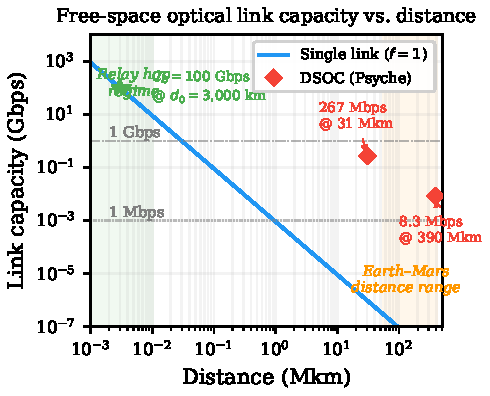
\includegraphics[width=0.75\columnwidth]{figures/link-capacity-vs-distance.pdf}
  \caption{Free-space optical link capacity vs.\ distance for a single
    DSOC-class terminal ($f = 1$, $K = 9 \times 10^{8}\Gbps\cdot\text{km}^2$).
    The DSOC data points are from NASA's Psyche
    mission~\cite{dsoc2024}. The shaded region marks the Earth--Mars
    distance range. A relay chain keeps every hop in the high-capacity regime
    (left of the plot), avoiding the interplanetary penalty entirely.}
  \label{fig:link-capacity-vs-distance}
\end{figure}

We adopt the many-satellite relay architecture for the remainder of this paper.
The next question---how to arrange those satellites---is addressed in
\cref{sec:topology}.
